% Options for packages loaded elsewhere
\PassOptionsToPackage{unicode}{hyperref}
\PassOptionsToPackage{hyphens}{url}
\PassOptionsToPackage{dvipsnames,svgnames*,x11names*}{xcolor}
%
\documentclass[
  ignorenonframetext,
]{beamer}
\usepackage{pgfpages}
\setbeamertemplate{caption}[numbered]
\setbeamertemplate{caption label separator}{: }
\setbeamercolor{caption name}{fg=normal text.fg}
\beamertemplatenavigationsymbolsempty
% Prevent slide breaks in the middle of a paragraph
\widowpenalties 1 10000
\raggedbottom
\setbeamertemplate{part page}{
  \centering
  \begin{beamercolorbox}[sep=16pt,center]{part title}
    \usebeamerfont{part title}\insertpart\par
  \end{beamercolorbox}
}
\setbeamertemplate{section page}{
  \centering
  \begin{beamercolorbox}[sep=12pt,center]{part title}
    \usebeamerfont{section title}\insertsection\par
  \end{beamercolorbox}
}
\setbeamertemplate{subsection page}{
  \centering
  \begin{beamercolorbox}[sep=8pt,center]{part title}
    \usebeamerfont{subsection title}\insertsubsection\par
  \end{beamercolorbox}
}
\AtBeginPart{
  \frame{\partpage}
}
\AtBeginSection{
  \ifbibliography
  \else
    \frame{\sectionpage}
  \fi
}
\AtBeginSubsection{
  \frame{\subsectionpage}
}
\usepackage{lmodern}
\usepackage{amssymb,amsmath}
\usepackage{ifxetex,ifluatex}
\ifnum 0\ifxetex 1\fi\ifluatex 1\fi=0 % if pdftex
  \usepackage[T1]{fontenc}
  \usepackage[utf8]{inputenc}
  \usepackage{textcomp} % provide euro and other symbols
\else % if luatex or xetex
  \usepackage{unicode-math}
  \defaultfontfeatures{Scale=MatchLowercase}
  \defaultfontfeatures[\rmfamily]{Ligatures=TeX,Scale=1}
\fi
\usetheme[]{AnnArbor}
\usecolortheme{dove}
% Use upquote if available, for straight quotes in verbatim environments
\IfFileExists{upquote.sty}{\usepackage{upquote}}{}
\IfFileExists{microtype.sty}{% use microtype if available
  \usepackage[]{microtype}
  \UseMicrotypeSet[protrusion]{basicmath} % disable protrusion for tt fonts
}{}
\makeatletter
\@ifundefined{KOMAClassName}{% if non-KOMA class
  \IfFileExists{parskip.sty}{%
    \usepackage{parskip}
  }{% else
    \setlength{\parindent}{0pt}
    \setlength{\parskip}{6pt plus 2pt minus 1pt}}
}{% if KOMA class
  \KOMAoptions{parskip=half}}
\makeatother
\usepackage{xcolor}
\IfFileExists{xurl.sty}{\usepackage{xurl}}{} % add URL line breaks if available
\IfFileExists{bookmark.sty}{\usepackage{bookmark}}{\usepackage{hyperref}}
\hypersetup{
  pdftitle={Statistical Inference: matched pairs and normal quantile plot},
  colorlinks=true,
  linkcolor=Maroon,
  filecolor=Maroon,
  citecolor=Blue,
  urlcolor=blue,
  pdfcreator={LaTeX via pandoc}}
\urlstyle{same} % disable monospaced font for URLs
\newif\ifbibliography
\usepackage{color}
\usepackage{fancyvrb}
\newcommand{\VerbBar}{|}
\newcommand{\VERB}{\Verb[commandchars=\\\{\}]}
\DefineVerbatimEnvironment{Highlighting}{Verbatim}{commandchars=\\\{\}}
% Add ',fontsize=\small' for more characters per line
\usepackage{framed}
\definecolor{shadecolor}{RGB}{248,248,248}
\newenvironment{Shaded}{\begin{snugshade}}{\end{snugshade}}
\newcommand{\AlertTok}[1]{\textcolor[rgb]{0.94,0.16,0.16}{#1}}
\newcommand{\AnnotationTok}[1]{\textcolor[rgb]{0.56,0.35,0.01}{\textbf{\textit{#1}}}}
\newcommand{\AttributeTok}[1]{\textcolor[rgb]{0.77,0.63,0.00}{#1}}
\newcommand{\BaseNTok}[1]{\textcolor[rgb]{0.00,0.00,0.81}{#1}}
\newcommand{\BuiltInTok}[1]{#1}
\newcommand{\CharTok}[1]{\textcolor[rgb]{0.31,0.60,0.02}{#1}}
\newcommand{\CommentTok}[1]{\textcolor[rgb]{0.56,0.35,0.01}{\textit{#1}}}
\newcommand{\CommentVarTok}[1]{\textcolor[rgb]{0.56,0.35,0.01}{\textbf{\textit{#1}}}}
\newcommand{\ConstantTok}[1]{\textcolor[rgb]{0.00,0.00,0.00}{#1}}
\newcommand{\ControlFlowTok}[1]{\textcolor[rgb]{0.13,0.29,0.53}{\textbf{#1}}}
\newcommand{\DataTypeTok}[1]{\textcolor[rgb]{0.13,0.29,0.53}{#1}}
\newcommand{\DecValTok}[1]{\textcolor[rgb]{0.00,0.00,0.81}{#1}}
\newcommand{\DocumentationTok}[1]{\textcolor[rgb]{0.56,0.35,0.01}{\textbf{\textit{#1}}}}
\newcommand{\ErrorTok}[1]{\textcolor[rgb]{0.64,0.00,0.00}{\textbf{#1}}}
\newcommand{\ExtensionTok}[1]{#1}
\newcommand{\FloatTok}[1]{\textcolor[rgb]{0.00,0.00,0.81}{#1}}
\newcommand{\FunctionTok}[1]{\textcolor[rgb]{0.00,0.00,0.00}{#1}}
\newcommand{\ImportTok}[1]{#1}
\newcommand{\InformationTok}[1]{\textcolor[rgb]{0.56,0.35,0.01}{\textbf{\textit{#1}}}}
\newcommand{\KeywordTok}[1]{\textcolor[rgb]{0.13,0.29,0.53}{\textbf{#1}}}
\newcommand{\NormalTok}[1]{#1}
\newcommand{\OperatorTok}[1]{\textcolor[rgb]{0.81,0.36,0.00}{\textbf{#1}}}
\newcommand{\OtherTok}[1]{\textcolor[rgb]{0.56,0.35,0.01}{#1}}
\newcommand{\PreprocessorTok}[1]{\textcolor[rgb]{0.56,0.35,0.01}{\textit{#1}}}
\newcommand{\RegionMarkerTok}[1]{#1}
\newcommand{\SpecialCharTok}[1]{\textcolor[rgb]{0.00,0.00,0.00}{#1}}
\newcommand{\SpecialStringTok}[1]{\textcolor[rgb]{0.31,0.60,0.02}{#1}}
\newcommand{\StringTok}[1]{\textcolor[rgb]{0.31,0.60,0.02}{#1}}
\newcommand{\VariableTok}[1]{\textcolor[rgb]{0.00,0.00,0.00}{#1}}
\newcommand{\VerbatimStringTok}[1]{\textcolor[rgb]{0.31,0.60,0.02}{#1}}
\newcommand{\WarningTok}[1]{\textcolor[rgb]{0.56,0.35,0.01}{\textbf{\textit{#1}}}}
\usepackage{longtable,booktabs}
\usepackage{caption}
% Make caption package work with longtable
\makeatletter
\def\fnum@table{\tablename~\thetable}
\makeatother
\usepackage{graphicx}
\makeatletter
\def\maxwidth{\ifdim\Gin@nat@width>\linewidth\linewidth\else\Gin@nat@width\fi}
\def\maxheight{\ifdim\Gin@nat@height>\textheight\textheight\else\Gin@nat@height\fi}
\makeatother
% Scale images if necessary, so that they will not overflow the page
% margins by default, and it is still possible to overwrite the defaults
% using explicit options in \includegraphics[width, height, ...]{}
\setkeys{Gin}{width=\maxwidth,height=\maxheight,keepaspectratio}
% Set default figure placement to htbp
\makeatletter
\def\fps@figure{htbp}
\makeatother
\setlength{\emergencystretch}{3em} % prevent overfull lines
\providecommand{\tightlist}{%
  \setlength{\itemsep}{0pt}\setlength{\parskip}{0pt}}
\setcounter{secnumdepth}{-\maxdimen} % remove section numbering
\usepackage{multicol}

\title{Statistical Inference: matched pairs and normal quantile plot}
\author{}
\date{\vspace{-2.5em}}

\begin{document}
\frame{\titlepage}

\begin{frame}[fragile]
knitr::opts\_chunk\(set(fig.height = 5) # knitr::opts_chunk\)set(echo =
FALSE) options(width=52) knitr::opts\_chunk\$set(dev = `pdf')

\begin{verbatim}






## Matched pairs

Some data: 

\centering{
  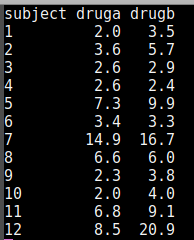
\includegraphics[height=0.7\textheight]{Screenshot_2019-04-26_13-41-29}
}


## Matched pairs data
- Data are comparison of 2 drugs for effectiveness at reducing pain.

     - 12 subjects (cases) were arthritis sufferers
     - Response is #hours of pain relief from each drug.
      
- In reading example, each child tried only one reading method.
- But here, each subject tried out both drugs, giving us two
measurements.

    - Possible because, if you wait long enough, one drug has no influence
over effect of other.
    - Advantage: focused comparison of drugs. Compare one drug with
another on same person, removes a lot of variability due to differences between people. 
    - Matched pairs, requires different analysis.
      
- Design: randomly choose 6 of 12 subjects to get drug A first, other 6
get drug B first.

## Paired t test: reading the data
Values aligned in columns:  


```r
my_url <- "http://www.utsc.utoronto.ca/~butler/c32/analgesic.txt"
pain <- read_table(my_url)
\end{verbatim}

\begin{verbatim}
## 
## -- Column specification --------------------------------------------------------
## cols(
##   subject = col_double(),
##   druga = col_double(),
##   drugb = col_double()
## )
\end{verbatim}
\end{frame}

\begin{frame}[fragile]{The data}
\protect\hypertarget{the-data}{}
\begin{Shaded}
\begin{Highlighting}[]
\NormalTok{pain}
\end{Highlighting}
\end{Shaded}

\begin{longtable}[]{@{}rrr@{}}
\toprule
subject & druga & drugb\tabularnewline
\midrule
\endhead
1 & 2.0 & 3.5\tabularnewline
2 & 3.6 & 5.7\tabularnewline
3 & 2.6 & 2.9\tabularnewline
4 & 2.6 & 2.4\tabularnewline
5 & 7.3 & 9.9\tabularnewline
6 & 3.4 & 3.3\tabularnewline
7 & 14.9 & 16.7\tabularnewline
8 & 6.6 & 6.0\tabularnewline
9 & 2.3 & 3.8\tabularnewline
10 & 2.0 & 4.0\tabularnewline
11 & 6.8 & 9.1\tabularnewline
12 & 8.5 & 20.9\tabularnewline
\bottomrule
\end{longtable}
\end{frame}

\begin{frame}[fragile]{Paired \emph{t}-test}
\protect\hypertarget{paired-t-test}{}
\small

\begin{Shaded}
\begin{Highlighting}[]
\KeywordTok{with}\NormalTok{(pain, }\KeywordTok{t.test}\NormalTok{(druga, drugb, }\DataTypeTok{paired =}\NormalTok{ T))}
\end{Highlighting}
\end{Shaded}

\begin{verbatim}
## 
##  Paired t-test
## 
## data:  druga and drugb
## t = -2.1677, df = 11, p-value = 0.05299
## alternative hypothesis: true difference in means is not equal to 0
## 95 percent confidence interval:
##  -4.29941513  0.03274847
## sample estimates:
## mean of the differences 
##               -2.133333
\end{verbatim}

\normalsize

\begin{itemize}
\tightlist
\item
  P-value is 0.053.
\item
  Not quite evidence of difference between drugs.
\end{itemize}
\end{frame}

\begin{frame}[fragile]{t-testing the differences}
\protect\hypertarget{t-testing-the-differences}{}
\begin{itemize}
\tightlist
\item
  Likewise, you can calculate the differences yourself and do a 1-sample
  t-test on them.
\item
  First calculate a column of differences:
\end{itemize}

\footnotesize

\begin{Shaded}
\begin{Highlighting}[]
\NormalTok{(pain }\OperatorTok{\%\textgreater{}\%}\StringTok{ }\KeywordTok{mutate}\NormalTok{(}\DataTypeTok{diff=}\NormalTok{druga}\OperatorTok{{-}}\NormalTok{drugb) {-}\textgreater{}}\StringTok{ }\NormalTok{pain)}
\end{Highlighting}
\end{Shaded}

\begin{longtable}[]{@{}rrrr@{}}
\toprule
subject & druga & drugb & diff\tabularnewline
\midrule
\endhead
1 & 2.0 & 3.5 & -1.5\tabularnewline
2 & 3.6 & 5.7 & -2.1\tabularnewline
3 & 2.6 & 2.9 & -0.3\tabularnewline
4 & 2.6 & 2.4 & 0.2\tabularnewline
5 & 7.3 & 9.9 & -2.6\tabularnewline
6 & 3.4 & 3.3 & 0.1\tabularnewline
7 & 14.9 & 16.7 & -1.8\tabularnewline
8 & 6.6 & 6.0 & 0.6\tabularnewline
9 & 2.3 & 3.8 & -1.5\tabularnewline
10 & 2.0 & 4.0 & -2.0\tabularnewline
11 & 6.8 & 9.1 & -2.3\tabularnewline
12 & 8.5 & 20.9 & -12.4\tabularnewline
\bottomrule
\end{longtable}

\normalsize
\end{frame}

\begin{frame}[fragile]{t-test on the differences}
\protect\hypertarget{t-test-on-the-differences}{}
\begin{itemize}
\tightlist
\item
  then throw them into t.test, testing that the mean is zero, with same
  result as before:
\end{itemize}

\begin{Shaded}
\begin{Highlighting}[]
\KeywordTok{with}\NormalTok{(pain,}\KeywordTok{t.test}\NormalTok{(diff,}\DataTypeTok{mu=}\DecValTok{0}\NormalTok{))}
\end{Highlighting}
\end{Shaded}

\begin{verbatim}
## 
##  One Sample t-test
## 
## data:  diff
## t = -2.1677, df = 11, p-value = 0.05299
## alternative hypothesis: true mean is not equal to 0
## 95 percent confidence interval:
##  -4.29941513  0.03274847
## sample estimates:
## mean of x 
## -2.133333
\end{verbatim}
\end{frame}

\begin{frame}{Assessing normality}
\protect\hypertarget{assessing-normality}{}
\begin{itemize}
\tightlist
\item
  1-sample and 2-sample t-tests assume (each) group normally
  distributed.
\item
  Matched pairs analyses assume (theoretically) that differences
  normally distributed.
\item
  Though we know that t-tests generally behave well even without
  normality.
\item
  How to assess normality? A normal quantile plot.

  \begin{itemize}
  \tightlist
  \item
    Idea: scatter of points should follow the straight line, without
    curving.
  \item
    Outliers show up at bottom left or top right of plot as points off
    the line.
  \end{itemize}
\end{itemize}
\end{frame}

\begin{frame}[fragile]{The normal quantile plot}
\protect\hypertarget{the-normal-quantile-plot}{}
\begin{itemize}
\tightlist
\item
  of differences from matched pairs data
\end{itemize}

\begin{Shaded}
\begin{Highlighting}[]
\KeywordTok{ggplot}\NormalTok{(pain,}\KeywordTok{aes}\NormalTok{(}\DataTypeTok{sample=}\NormalTok{diff))}\OperatorTok{+}\KeywordTok{stat\_qq}\NormalTok{()}\OperatorTok{+}\KeywordTok{stat\_qq\_line}\NormalTok{()}
\end{Highlighting}
\end{Shaded}

\includegraphics{inference_4b_R_slides_files/figure-beamer/unnamed-chunk-9-1.pdf}

\begin{itemize}
\tightlist
\item
  Points should follow the straight line. Bottom left one way off, so
  normality questionable here: outlier.
\end{itemize}
\end{frame}

\begin{frame}{More normal quantile plots}
\protect\hypertarget{more-normal-quantile-plots}{}
\begin{itemize}
\tightlist
\item
  How straight does a normal quantile plot have to be?
\item
  There is randomness in real data, so even a normal quantile plot from
  normal data won't look perfectly straight.
\item
  With a small sample, can look not very straight even from normal data.
\item
  Looking for systematic departure from a straight line; random wiggles
  ought not to concern us.
\item
  Look at some examples where we know the answer, so that we can see
  what to expect.
\end{itemize}
\end{frame}

\begin{frame}[fragile]{Normal data, large sample}
\protect\hypertarget{normal-data-large-sample}{}
\begin{Shaded}
\begin{Highlighting}[]
\NormalTok{d=}\KeywordTok{tibble}\NormalTok{(}\DataTypeTok{x=}\KeywordTok{rnorm}\NormalTok{(}\DecValTok{200}\NormalTok{))}
\KeywordTok{ggplot}\NormalTok{(d,}\KeywordTok{aes}\NormalTok{(}\DataTypeTok{x=}\NormalTok{x))}\OperatorTok{+}\KeywordTok{geom\_histogram}\NormalTok{(}\DataTypeTok{bins=}\DecValTok{10}\NormalTok{)}
\end{Highlighting}
\end{Shaded}

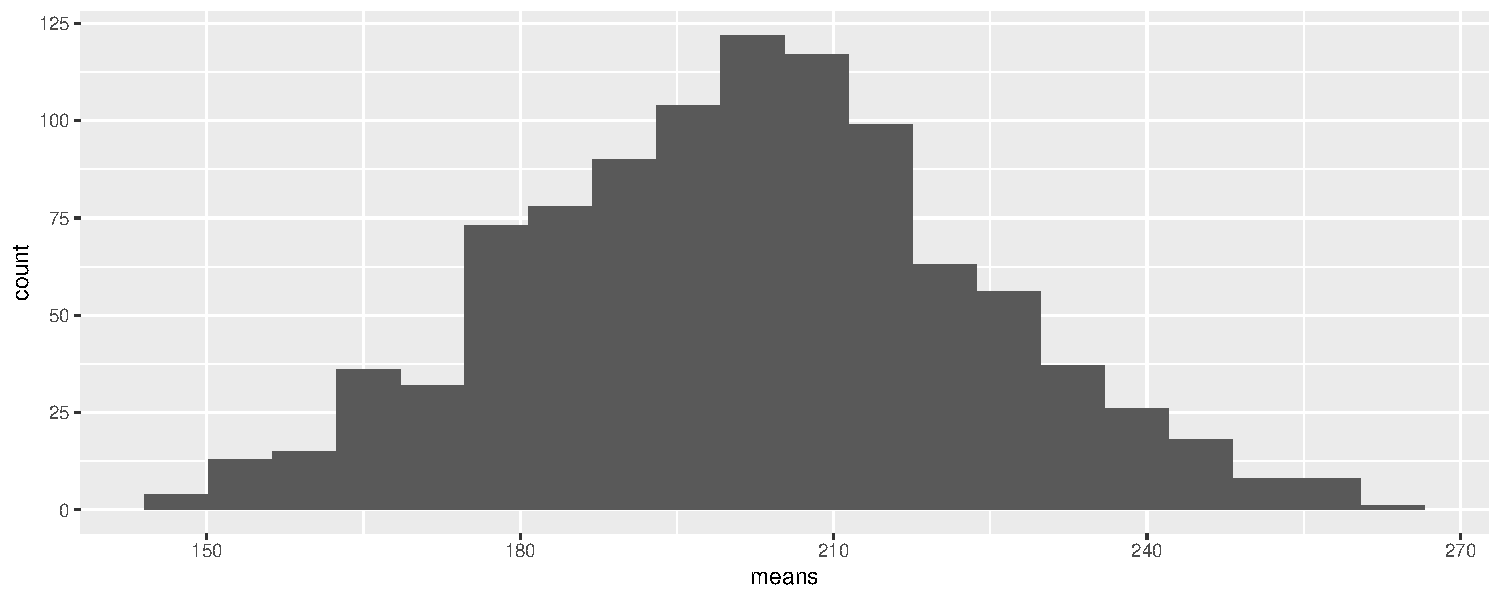
\includegraphics{inference_4b_R_slides_files/figure-beamer/unnamed-chunk-10-1.pdf}
\end{frame}

\begin{frame}[fragile]{The normal quantile plot}
\protect\hypertarget{the-normal-quantile-plot-1}{}
\begin{Shaded}
\begin{Highlighting}[]
\KeywordTok{ggplot}\NormalTok{(d,}\KeywordTok{aes}\NormalTok{(}\DataTypeTok{sample=}\NormalTok{x))}\OperatorTok{+}\KeywordTok{stat\_qq}\NormalTok{()}\OperatorTok{+}\KeywordTok{stat\_qq\_line}\NormalTok{()}
\end{Highlighting}
\end{Shaded}

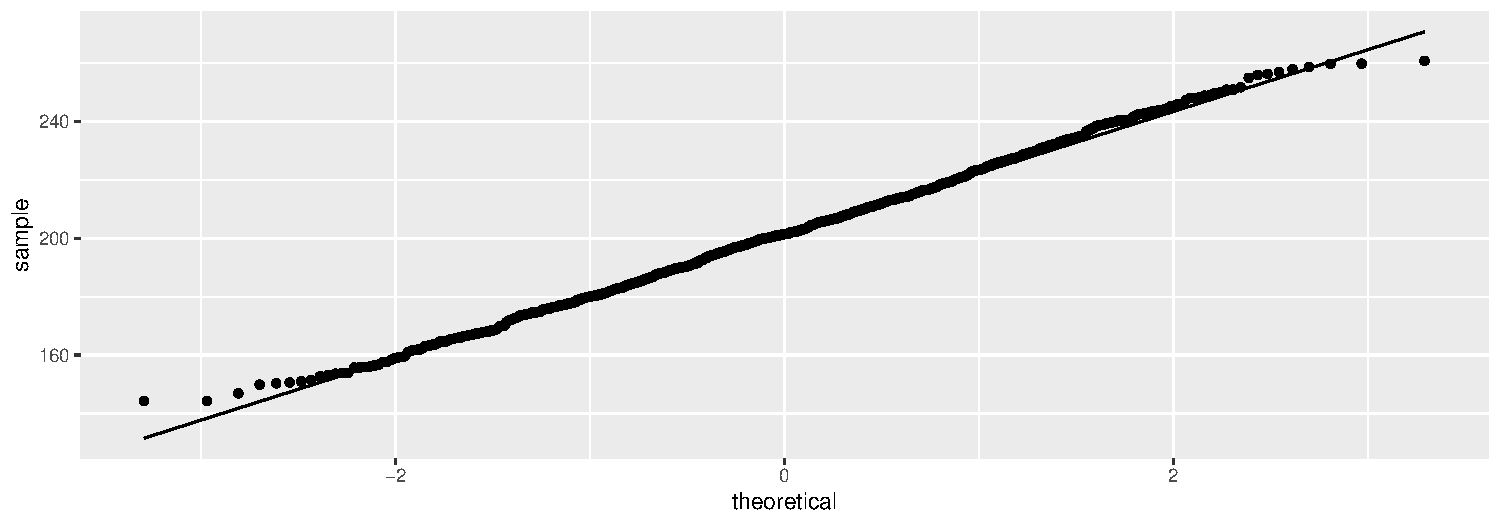
\includegraphics{inference_4b_R_slides_files/figure-beamer/unnamed-chunk-11-1.pdf}
\end{frame}

\begin{frame}[fragile]{Normal data, small sample}
\protect\hypertarget{normal-data-small-sample}{}
\begin{itemize}
\tightlist
\item
  Not so convincingly normal, but not obviously skewed:
\end{itemize}

\begin{Shaded}
\begin{Highlighting}[]
\NormalTok{d=}\KeywordTok{tibble}\NormalTok{(}\DataTypeTok{x=}\KeywordTok{rnorm}\NormalTok{(}\DecValTok{20}\NormalTok{))}
\KeywordTok{ggplot}\NormalTok{(d,}\KeywordTok{aes}\NormalTok{(}\DataTypeTok{x=}\NormalTok{x))}\OperatorTok{+}\KeywordTok{geom\_histogram}\NormalTok{(}\DataTypeTok{bins=}\DecValTok{5}\NormalTok{)}
\end{Highlighting}
\end{Shaded}

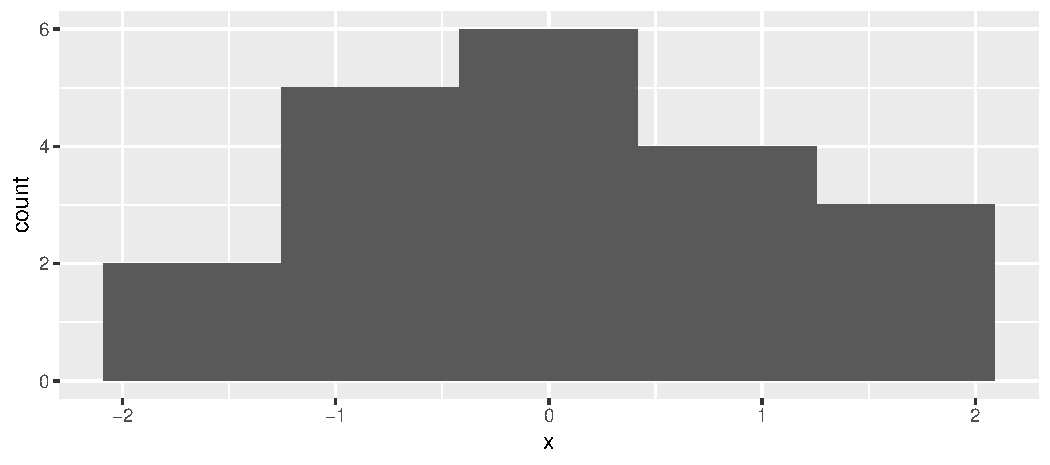
\includegraphics{inference_4b_R_slides_files/figure-beamer/normal-small-1.pdf}
\end{frame}

\begin{frame}[fragile]{The normal quantile plot}
\protect\hypertarget{the-normal-quantile-plot-2}{}
Good, apart from the highest and lowest points being slightly off. I'd
call this good:

\begin{Shaded}
\begin{Highlighting}[]
\KeywordTok{ggplot}\NormalTok{(d,}\KeywordTok{aes}\NormalTok{(}\DataTypeTok{sample=}\NormalTok{x))}\OperatorTok{+}\KeywordTok{stat\_qq}\NormalTok{()}\OperatorTok{+}\KeywordTok{stat\_qq\_line}\NormalTok{()}
\end{Highlighting}
\end{Shaded}

\includegraphics{inference_4b_R_slides_files/figure-beamer/unnamed-chunk-13-1.pdf}
\end{frame}

\begin{frame}[fragile]{Chi-squared data, \emph{df} = 10}
\protect\hypertarget{chi-squared-data-df-10}{}
Somewhat skewed to right:

\begin{Shaded}
\begin{Highlighting}[]
\NormalTok{d=}\KeywordTok{tibble}\NormalTok{(}\DataTypeTok{x=}\KeywordTok{rchisq}\NormalTok{(}\DecValTok{100}\NormalTok{,}\DecValTok{10}\NormalTok{))}
\KeywordTok{ggplot}\NormalTok{(d,}\KeywordTok{aes}\NormalTok{(}\DataTypeTok{x=}\NormalTok{x))}\OperatorTok{+}\KeywordTok{geom\_histogram}\NormalTok{(}\DataTypeTok{bins=}\DecValTok{10}\NormalTok{)}
\end{Highlighting}
\end{Shaded}

\includegraphics{inference_4b_R_slides_files/figure-beamer/unnamed-chunk-14-1.pdf}
\end{frame}

\begin{frame}[fragile]{The normal quantile plot}
\protect\hypertarget{the-normal-quantile-plot-3}{}
Somewhat opening-up curve:

\begin{Shaded}
\begin{Highlighting}[]
\KeywordTok{ggplot}\NormalTok{(d,}\KeywordTok{aes}\NormalTok{(}\DataTypeTok{sample=}\NormalTok{x))}\OperatorTok{+}\KeywordTok{stat\_qq}\NormalTok{()}\OperatorTok{+}\KeywordTok{stat\_qq\_line}\NormalTok{()}
\end{Highlighting}
\end{Shaded}

\includegraphics{inference_4b_R_slides_files/figure-beamer/unnamed-chunk-15-1.pdf}
\end{frame}

\begin{frame}[fragile]{Chi-squared data, df = 3}
\protect\hypertarget{chi-squared-data-df-3}{}
Definitely skewed to right:

\begin{Shaded}
\begin{Highlighting}[]
\NormalTok{d=}\KeywordTok{tibble}\NormalTok{(}\DataTypeTok{x=}\KeywordTok{rchisq}\NormalTok{(}\DecValTok{100}\NormalTok{,}\DecValTok{3}\NormalTok{))}
\KeywordTok{ggplot}\NormalTok{(d,}\KeywordTok{aes}\NormalTok{(}\DataTypeTok{x=}\NormalTok{x))}\OperatorTok{+}\KeywordTok{geom\_histogram}\NormalTok{(}\DataTypeTok{bins=}\DecValTok{10}\NormalTok{)}
\end{Highlighting}
\end{Shaded}

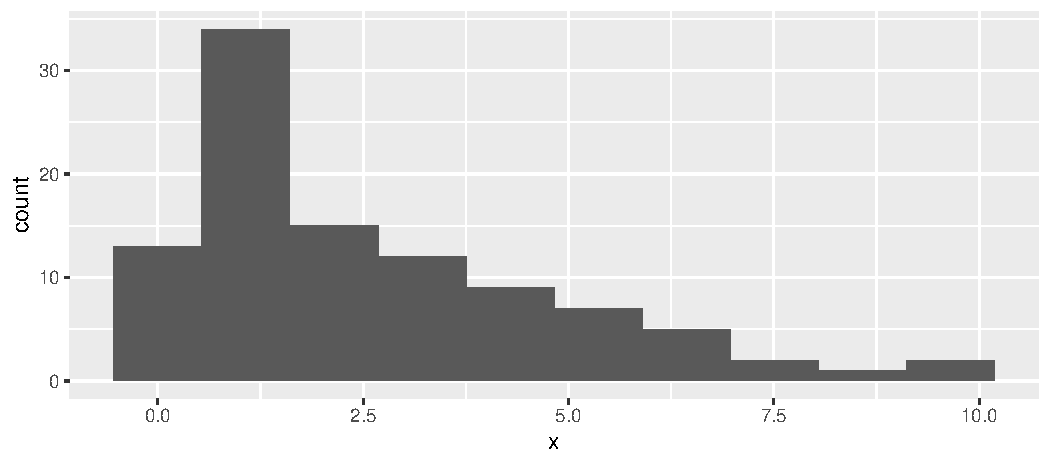
\includegraphics{inference_4b_R_slides_files/figure-beamer/chisq-small-df-1.pdf}
\end{frame}

\begin{frame}[fragile]{The normal quantile plot}
\protect\hypertarget{the-normal-quantile-plot-4}{}
Clear upward-opening curve:

\begin{Shaded}
\begin{Highlighting}[]
\KeywordTok{ggplot}\NormalTok{(d,}\KeywordTok{aes}\NormalTok{(}\DataTypeTok{sample=}\NormalTok{x))}\OperatorTok{+}\KeywordTok{stat\_qq}\NormalTok{()}\OperatorTok{+}\KeywordTok{stat\_qq\_line}\NormalTok{()}
\end{Highlighting}
\end{Shaded}

\includegraphics{inference_4b_R_slides_files/figure-beamer/unnamed-chunk-16-1.pdf}
\end{frame}

\begin{frame}[fragile]{t-distributed data, df = 3}
\protect\hypertarget{t-distributed-data-df-3}{}
Long tails (or a very sharp peak):

\begin{Shaded}
\begin{Highlighting}[]
\NormalTok{d=}\KeywordTok{tibble}\NormalTok{(}\DataTypeTok{x=}\KeywordTok{rt}\NormalTok{(}\DecValTok{300}\NormalTok{,}\DecValTok{3}\NormalTok{))}
\KeywordTok{ggplot}\NormalTok{(d,}\KeywordTok{aes}\NormalTok{(}\DataTypeTok{x=}\NormalTok{x))}\OperatorTok{+}\KeywordTok{geom\_histogram}\NormalTok{(}\DataTypeTok{bins=}\DecValTok{10}\NormalTok{)}
\end{Highlighting}
\end{Shaded}

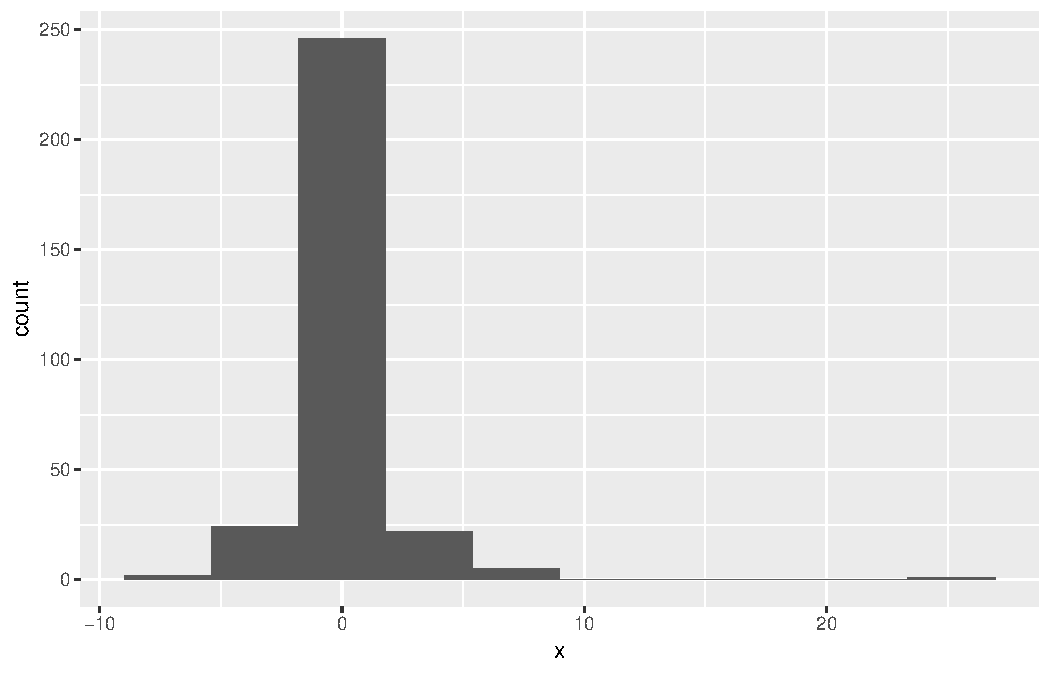
\includegraphics{inference_4b_R_slides_files/figure-beamer/t-small-1.pdf}
\end{frame}

\begin{frame}[fragile]{The normal quantile plot}
\protect\hypertarget{the-normal-quantile-plot-5}{}
Low values too low and high values too high for normal.

\begin{Shaded}
\begin{Highlighting}[]
\KeywordTok{ggplot}\NormalTok{(d,}\KeywordTok{aes}\NormalTok{(}\DataTypeTok{sample=}\NormalTok{x))}\OperatorTok{+}\KeywordTok{stat\_qq}\NormalTok{()}\OperatorTok{+}\KeywordTok{stat\_qq\_line}\NormalTok{()}
\end{Highlighting}
\end{Shaded}

\includegraphics{inference_4b_R_slides_files/figure-beamer/unnamed-chunk-17-1.pdf}
\end{frame}

\begin{frame}[fragile]{Our pain-relief data}
\protect\hypertarget{our-pain-relief-data}{}
\begin{Shaded}
\begin{Highlighting}[]
\KeywordTok{ggplot}\NormalTok{(pain,}\KeywordTok{aes}\NormalTok{(}\DataTypeTok{sample=}\NormalTok{diff))}\OperatorTok{+}\KeywordTok{stat\_qq}\NormalTok{()}\OperatorTok{+}\KeywordTok{stat\_qq\_line}\NormalTok{()}
\end{Highlighting}
\end{Shaded}

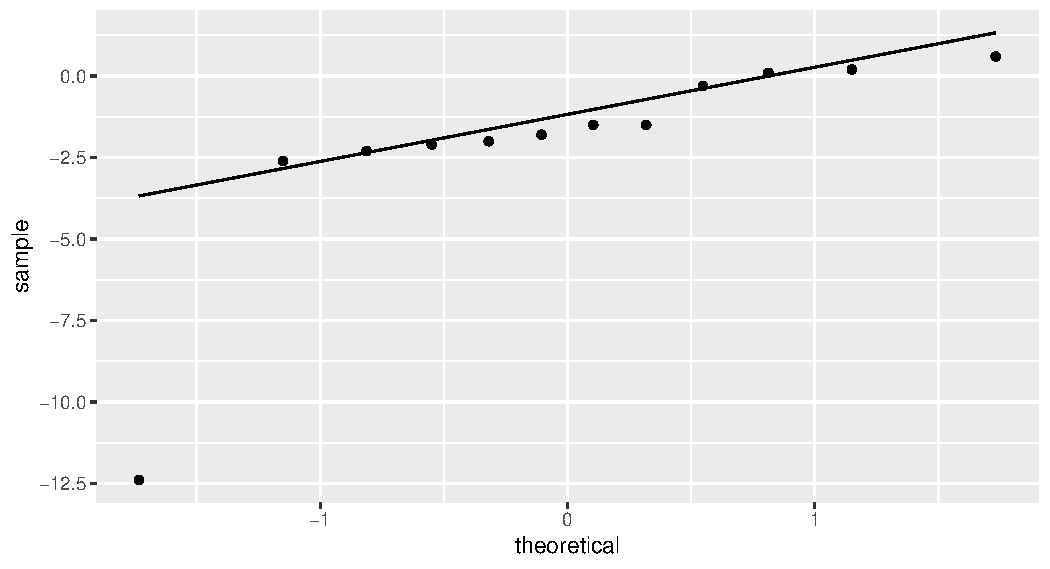
\includegraphics{inference_4b_R_slides_files/figure-beamer/pain-relief-qq-1.pdf}
\end{frame}

\begin{frame}{Comments}
\protect\hypertarget{comments}{}
\begin{itemize}
\tightlist
\item
  Definitely not normal. What to do?
\item
  Sign test on differences, null median 0.
\end{itemize}
\end{frame}

\begin{frame}[fragile]{Sign test}
\protect\hypertarget{sign-test}{}
\begin{itemize}
\tightlist
\item
  Most easily: calculate differences in data frame, then use
  \texttt{smmr}.
\item
  Null median difference is 0:
\end{itemize}

\begin{Shaded}
\begin{Highlighting}[]
\NormalTok{pain }\OperatorTok{\%\textgreater{}\%}\StringTok{ }\KeywordTok{mutate}\NormalTok{(}\DataTypeTok{mydiff=}\NormalTok{druga}\OperatorTok{{-}}\NormalTok{drugb) }\OperatorTok{\%\textgreater{}\%}
\KeywordTok{sign\_test}\NormalTok{(mydiff,}\DecValTok{0}\NormalTok{)}
\end{Highlighting}
\end{Shaded}

\begin{verbatim}
## $above_below
## below above 
##     9     3 
## 
## $p_values
##   alternative    p_value
## 1       lower 0.07299805
## 2       upper 0.98071289
## 3   two-sided 0.14599609
\end{verbatim}
\end{frame}

\begin{frame}[fragile]{Comments}
\protect\hypertarget{comments-1}{}
\begin{itemize}
\tightlist
\item
  P-value 0.1460. No evidence that the drugs are different.
\item
  Since we are working in a pipeline, input data frame to
  \texttt{sign\_test} is ``whatever came out of previous step''.
\end{itemize}
\end{frame}

\begin{frame}[fragile]{(Some of) the kids' reading data, again}
\protect\hypertarget{some-of-the-kids-reading-data-again}{}
\begin{verbatim}
## 
## -- Column specification --------------------------------------------------------
## cols(
##   group = col_character(),
##   score = col_double()
## )
\end{verbatim}

\begin{Shaded}
\begin{Highlighting}[]
\NormalTok{kids }\OperatorTok{\%\textgreater{}\%}\StringTok{ }\KeywordTok{slice\_sample}\NormalTok{(}\DataTypeTok{n=}\DecValTok{12}\NormalTok{)}
\end{Highlighting}
\end{Shaded}

\begin{longtable}[]{@{}lr@{}}
\toprule
group & score\tabularnewline
\midrule
\endhead
t & 44\tabularnewline
c & 26\tabularnewline
t & 59\tabularnewline
c & 55\tabularnewline
t & 62\tabularnewline
t & 43\tabularnewline
c & 10\tabularnewline
t & 57\tabularnewline
t & 67\tabularnewline
c & 28\tabularnewline
c & 42\tabularnewline
t & 33\tabularnewline
\bottomrule
\end{longtable}
\end{frame}

\begin{frame}{Where we were at}
\protect\hypertarget{where-we-were-at}{}
\begin{itemize}
\item
  21 kids in ``treatment'', new reading method; 23 in ``control'',
  standard reading method.
\item
  Assessing assumptions:

  \begin{itemize}
  \tightlist
  \item
    We did two-sample t-test (Satterthwaite-Welch) before.
  \item
    Assumes approx. normal data within each group.
  \item
    Does not assume equal spread.
  \item
    (Pooled t-test \emph{does} assume equal spread).
  \item
    Assess each group separately.
  \end{itemize}
\end{itemize}
\end{frame}

\begin{frame}[fragile]{Boxplots for reading data}
\protect\hypertarget{boxplots-for-reading-data}{}
\begin{Shaded}
\begin{Highlighting}[]
\KeywordTok{ggplot}\NormalTok{(kids,}\KeywordTok{aes}\NormalTok{(}\DataTypeTok{x=}\NormalTok{group,}\DataTypeTok{y=}\NormalTok{score))}\OperatorTok{+}\KeywordTok{geom\_boxplot}\NormalTok{()}
\end{Highlighting}
\end{Shaded}

\includegraphics{inference_4b_R_slides_files/figure-beamer/unnamed-chunk-21-1.pdf}
\end{frame}

\begin{frame}[fragile]{Facetted normal quantile plots}
\protect\hypertarget{facetted-normal-quantile-plots}{}
Done this way:

\begin{Shaded}
\begin{Highlighting}[]
\KeywordTok{ggplot}\NormalTok{(kids,}\KeywordTok{aes}\NormalTok{(}\DataTypeTok{sample=}\NormalTok{score))}\OperatorTok{+}\KeywordTok{stat\_qq}\NormalTok{()}\OperatorTok{+}\KeywordTok{stat\_qq\_line}\NormalTok{()}\OperatorTok{+}
\KeywordTok{facet\_wrap}\NormalTok{(}\OperatorTok{\textasciitilde{}}\NormalTok{group)}
\end{Highlighting}
\end{Shaded}

\includegraphics{inference_4b_R_slides_files/figure-beamer/unnamed-chunk-22-1.pdf}
\end{frame}

\begin{frame}{Comments}
\protect\hypertarget{comments-2}{}
\begin{itemize}
\tightlist
\item
  These plots show no problems with normality. Both groups are more or
  less symmetric/normal and there are no outliers.
\item
  Equal spreads questionable, but we don't need that.
\item
  Assess equal spreads by looking at \emph{slopes} of normal quantile
  plots.
\item
  We ought be happy with the (Welch) two-sample t-test (over)
\end{itemize}
\end{frame}

\begin{frame}[fragile]{Welch two-sample test}
\protect\hypertarget{welch-two-sample-test}{}
\begin{Shaded}
\begin{Highlighting}[]
\KeywordTok{t.test}\NormalTok{(score}\OperatorTok{\textasciitilde{}}\NormalTok{group,}\DataTypeTok{data=}\NormalTok{kids,}\DataTypeTok{alternative=}\StringTok{"less"}\NormalTok{)}
\end{Highlighting}
\end{Shaded}

\begin{verbatim}
## 
##  Welch Two Sample t-test
## 
## data:  score by group
## t = -2.3109, df = 37.855, p-value = 0.01319
## alternative hypothesis: true difference in means is less than 0
## 95 percent confidence interval:
##       -Inf -2.691293
## sample estimates:
## mean in group c mean in group t 
##        41.52174        51.47619
\end{verbatim}

from which we concluded that the new reading method really does help.
\end{frame}

\end{document}
